\documentclass[10pt, a4paper, twoside]{basestyle}
\usepackage{tkz-euclide}
\usetkzobj{all}
\usepackage[Mathematics]{semtex}
\usepackage{chngcntr}
\counterwithout{equation}{section}

%%%% Shorthands.

%%%% Title and authors.

\newcommand{\point}[1]{\mathrm{#1}}
\newcommand{\bipoint}[2]{\overrightarrow{\point #1 \point #2}}
\newcommand{\straightline}[2]{\point #1 \point #2}
\newcommand{\plane}[3]{\point #1 \point #2 \point #3}
\newcommand{\squarenorm}[1]{\scal{#1}{#1}}

\title{%
\textdisplay{%
Hiding Computations in Projection%
}%
}
\author{Pascal~Leroy (pleroy)}
\begin{document}
\maketitle
This document describes the computations that are performed by the method
VisibleSegments of class Perspective to determine the parts of a segment that
are hidden by a sphere when seen from a pinhole camera.

Figure~\ref{fig3d} illustrates an example of the problem.  The points drawn in
black define the problem: $\point A$ and $\point B$ are the extremities of the
segment; $\point C$ is the centre of the sphere; $R$ is the radius of the
sphere; and $\point K$ is the location of the camera.  The points drawn in red
will be computed as part of the resolution.  Of particular interest is the plane
$\plane KAB$, in which we willl do much of the analysis below.  The figure shows
the circle formed by the intersection of this plane with the sphere, as well as
$\point H$, the center of that circle and the projection of $\point C$ on
$\plane KAB$.
\begin{figure}[htb!]
\centering
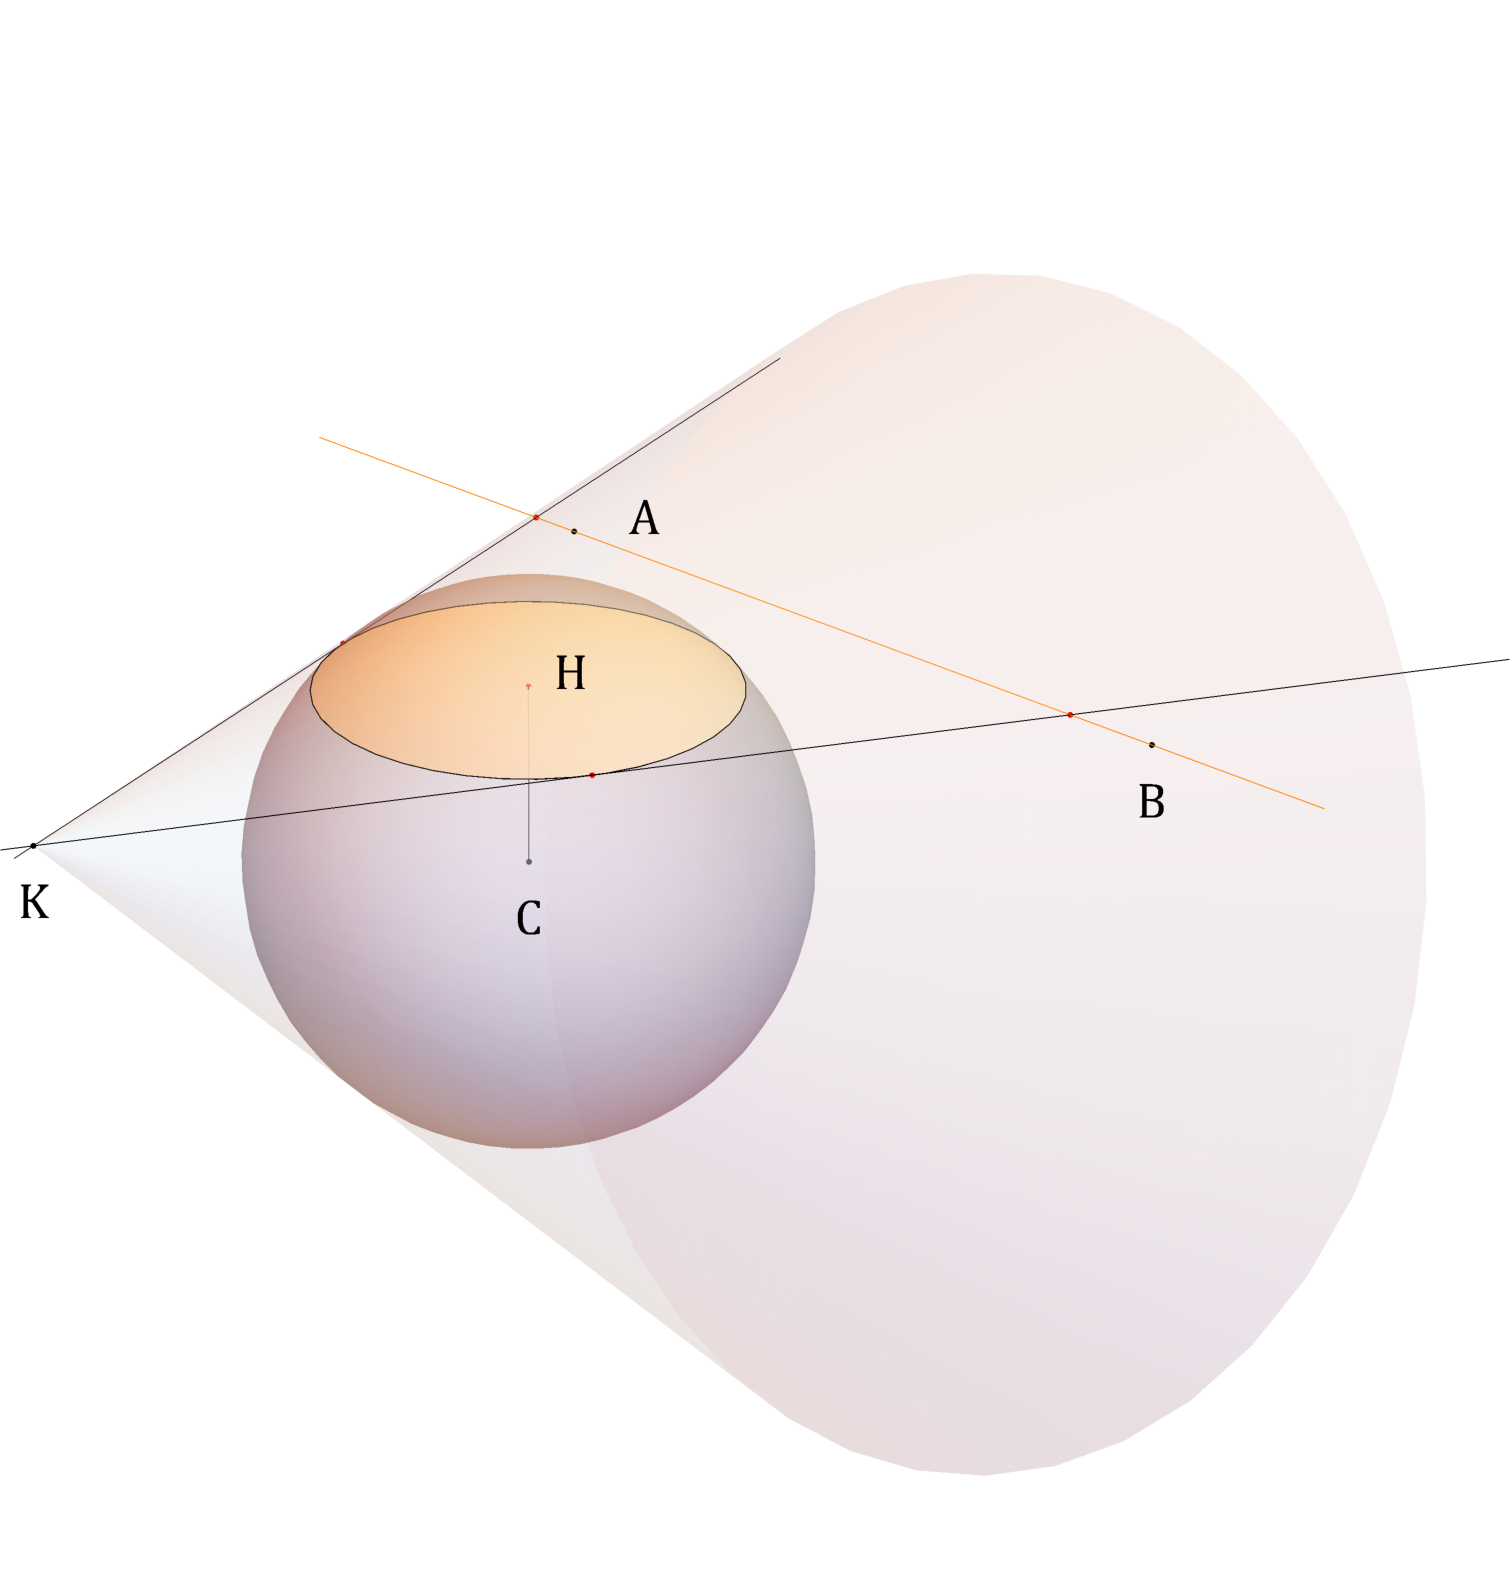
\includegraphics[scale=0.35]{Perspective-hiding-3d}
\caption{A 3-dimensional example.  In this case, the only segment visible from
$\point K$ is the part of $\straightline AB$ between $\point B$ and the red
point immediately to its left.\label{fig3d}}
\end{figure}

\subsection*{Camera inside the sphere}
We start our analysis by eliminating a case that would cause anomalies in the
analysis below.  If\[
\scal{\bipoint KC}{\bipoint KC} < R^2
\]
then the camera is inside the sphere and the segment is hidden irrespective of
its position.

\subsection*{Sphere and segment in distinct half-spaces}
Consider the plane containing $\point K$ and orthogonal to $\straightline KC$;
it separates the entire space into two half-spaces.  If the segment
$\straightline AB$ is entirely within the half-space that does not contain
$\point C$ then the segment is not hidden (remember that $\point K$ is not
inside the sphere).  This is the case if the following inequalities are both
true:
\begin{align*}
\scal{\bipoint KA}{\bipoint KC} &< 0\\
\scal{\bipoint KB}{\bipoint KC} &< 0\text.
\end{align*}

\subsection*{Projection of $\point C$ on $\plane KAB$}
For simplicity we will do the rest of our analysis in the plane $\plane KAB$ and
we will often use $\tuple{\bipoint KA, \bipoint KB}$ as a basis of that plane.
Let $\point H$ be the orthogonal projection of $\point C$ on $\plane KAB$.
and define $\ga$, $\gb$ to be its coordinates in
$\tuple{\bipoint KA, \bipoint KB}$
\[
\bipoint KH = \ga \bipoint KA + \gb \bipoint KB\text.
\]
Note that $\bipoint KH = \bipoint KC + \bipoint CH$. By definition,
$\bipoint CH$ is orthogonal to both $\bipoint KA$ and $\bipoint KB$:
\begin{align*}
\scal{\bipoint KA}{\bipoint CH} &= 0\\
\scal{\bipoint KB}{\bipoint CH} &= 0\text.
\end{align*}
Decomposing $\bipoint CH$ we obtain:
\begin{align*}
\scal{\bipoint KA}{\bipoint KH} &= \scal{\bipoint KA}{\bipoint KC}\\
\scal{\bipoint KB}{\bipoint KH} &= \scal{\bipoint KB}{\bipoint KC}\text.
\end{align*}
Expanding $\bipoint KH$ on the basis $\tuple{\bipoint KA, \bipoint KB}$ gives a
linear system of two equations with two unknowns:
\begin{align*}
\ga \scal{\bipoint KA}{\bipoint KA} + \gb \scal{\bipoint KA}{\bipoint KB}
    &= \scal{\bipoint KA}{\bipoint KC}\\
\ga \scal{\bipoint KA}{\bipoint KB} + \ga \scal{\bipoint KB}{\bipoint KB}
    &= \scal{\bipoint KB}{\bipoint KC}\text.
\end{align*}
The determinant of this system is\[
D = \pascal{\squarenorm{\bipoint KA}} \pascal{\squarenorm{\bipoint KB}} -
    \pascal{\scal{\bipoint KA}{\bipoint KB}}^2\text,
\]
which is non-zero if and only if $\point A \neq \point B$. The solutions are
thus:
\begin{align*}
\ga &= \frac
  {\pascal{\squarenorm{\bipoint KB}} \pascal{\scal{\bipoint KA}{\bipoint KC}} -
   \pascal{\scal{\bipoint KA}{\bipoint KB}}
   \pascal{\scal{\bipoint KB}{\bipoint KC}}}
  {D}\\
\gb &= \frac
  {\pascal{\squarenorm{\bipoint KA}} \pascal{\scal{\bipoint KB}{\bipoint KC}} -
   \pascal{\scal{\bipoint KA}{\bipoint KB}}
   \pascal{\scal{\bipoint KA}{\bipoint KC}}}
  {D}\text.
\end{align*}
Once $\bipoint KH$ is determined we can compute $\bipoint CH =
\bipoint KH - \bipoint KC$.  If $\squarenorm{\bipoint CH} \geq R^2$, the sphere
is either tangent to the plane $\plane KAB$ or doesn't intersect it. In these
cases, there is no hiding.

If the sphere intersects $\plane KAB$, then the intersection is a circle whose
radius we denote by $r$ in the rest of this analysis.  The radius is such that
$r^2 = R^2 - \squarenorm{\bipoint CH}$.

\subsection*{An optimization where the circle is outside the wedge $\plane KAB$}
\marginfig[Circle lying outside the wedge $\plane KAB$ on the side of
$\straightline KB$.\label{figOutside}]{
\begin{tikzpicture}[scale=0.5]
\tkzInit[ymin=-7,ymax=8,xmin=-1,xmax=9]
\tkzClip
\tkzDefPoint(3,5){A}
\tkzDefPoint(8,0){B}
\tkzDefPoint(4,-3){H}
\tkzDefPoint(0,0){K}

\tkzDefLine[orthogonal=through H](K,B) \tkzGetPoint{h1}
\tkzInterLL(H,h1)(K,B) \tkzGetPoint{N}

\tkzDefLine[parallel=through H](K,A) \tkzGetPoint{h2}
\tkzInterLL(H,h2)(K,B) \tkzGetPoint{M}

\tkzDefPointWith[linear,K=2](H,M) \tkzGetPoint{m}

\tkzDefPointBy[rotation=center H angle -130](N) \tkzGetPoint{r}

\tkzDrawPoints(A,B,H,K,M,N)
\tkzLabelPoint[left](A){$\point A$}
\tkzLabelPoint[above](B){$\point B$}
\tkzLabelPoint[left](H){$\point H$}
\tkzLabelPoint[above left](K){$\point K$}
\tkzLabelPoint[below right](M){$\point M$}
\tkzLabelPoint[above left](N){$\point N$}

\tkzDrawLine(K,A)
\tkzDrawLine(K,B)
\tkzDrawLine(H,N)
\tkzDrawLine[add=0.2 and 0.5](H,M)

\tkzDrawSegment[style=dashed](H,r)
\tkzLabelSegment[above right](H,r){$r$}

\tkzDrawCircle[R](H,3cm)

\tkzMarkRightAngle[size=0.5](H,N,M)
\tkzMarkAngle[size=0.5](B,K,A)
\tkzLabelAngle(A,K,B){$\gq$}
\tkzMarkAngle[size=0.5](B,M,m)
\tkzLabelAngle(B,M,m){$\gq$}

\end{tikzpicture}
}
A useful optimization at this stage is to determine if the circle intersects the
wedge $\plane KAB$.  If it does not, then there is no hiding and the segment
$\straightline AB$ is entirely visible.  This can happen because the circle is
away from the wedge on the side of $\straightline KA$ or because it is away from
the wedge on the side of $\straightline KB$.  Figure~\ref{figOutside}
illustrates the latter case: note that the circle must not intersect
$\straightline KB$, so the distance between $\point H$ and $\straightline KB$
must be at least $r$; the figure shows the case where the circle is tangent to
$\straightline KB$ at $\point N$, which is the one that interests us in this
section.

Observe that, if $\gq$ is the angle between $\bipoint KA$ and $\bipoint KB$, we
have
\[
\scal{\bipoint KA}{\bipoint KB} = \norm{\bipoint KA} \norm{\bipoint KB}
                                  \cos \gq
\]
Let $\point M$ be the point where $\point H$ projects on $\straightline KB$
parallel to $\straightline KA$.  Since $\ga$ and $\gb$ are the coordinates of
$\bipoint KH$ in the basis $\tuple{\bipoint KA, \bipoint KB}$, we
have
\begin{equation}
{\bipoint HM} = \ga {\bipoint KA} \label{eqnhm1}\text,
\end{equation}
and elementary trigonometry in the triangle $\plane HNM$ yields
\begin{equation}
\scal{\bipoint HM}{\bipoint HM} = \frac{r^2} {\sin^2 \gq} =
                                  \frac{r^2} {1 - \cos^2 \gq}
                                  \label{eqnhm2}\text.
\end{equation}
Eliminating $\bipoint HM$ between equations (\ref{eqnhm1}) and (\ref{eqnhm2}) we
obtain the following conditions on $\ga$ for $\point H$ to be outside the wedge
$\plane KAB$ on the side of $\straightline KB$:
\begin{align*}
\ga &\leq 0\\
\ga^2 &\geq r^2 \frac{\squarenorm{\bipoint KB}}
                     {\pascal{\squarenorm{\bipoint KA}}
                      \pascal{\squarenorm{\bipoint KB}} -
                     {\pascal{\scal{\bipoint KA}{\bipoint KB}}}^2}\text.
\end{align*}
It's straightforward to prove similar conditions on $\gb$ for the circle to be
outside the wedge $\plane KAB$ on the side of $\straightline KA$.

\subsection*{Construction of the cone}
\marginfig[Construction of $\point P$ and $\point P'$ and of the cone.
\label{figP}]{
\begin{tikzpicture}[scale=0.5]
\tkzInit[ymin=-5,ymax=10,xmin=-4,xmax=6]
\tkzClip
\tkzDefPoint(-3,9){A}
\tkzDefPoint(5.5,9){B}
\tkzDefPoint(2,5){H}
\tkzDefPoint(0,-4){K}

\tkzTangent[from with R=K](H,3cm) \tkzGetPoints{P'}{P}
\tkzInterLL(K,P)(A,B) \tkzGetPoint{Q}

\tkzDefPointBy[rotation=center H angle -130](P) \tkzGetPoint{r}

\tkzDrawPoints(A,B,H,K,P,P',Q)
\tkzLabelPoint[below left](A){$\point A$}
\tkzLabelPoint[above left](B){$\point B$}
\tkzLabelPoint[below](H){$\point H$}
\tkzLabelPoint[left](K){$\point K$}
\tkzLabelPoint[above left](P){$\point P$}
\tkzLabelPoint[below right](P'){$\point P'$}
\tkzLabelPoint[above right](Q){$\point Q$}

\tkzDrawLine[add=0.05 and 0.05](A,B)
\tkzDrawLine(H,P)
\tkzDrawLine(K,A)
\tkzDrawLine(K,B)
\tkzDrawLine(K,P')
\tkzDrawLine(K,Q)

\tkzDrawSegment[style=dashed](H,r)
\tkzLabelSegment[left](H,r){$r$}

\tkzDrawCircle[R](H,3cm)

\tkzMarkRightAngle[size=0.5](K,P,H)

\end{tikzpicture}
}
Remember that the circle of centre $\point H$ and radius $r$ is the intersection
of the sphere with the plane $\plane KAB$.  As shown on figure~\ref{fig3d},
hiding is determined by the cone of apex $\point K$ tangent to the sphere.  This
cone intersects $\plane KAB$ in two straight lines that go through $\point K$
and are tangent to the circle at points $\point P$ and $\point P'$.  In this
section we are going to determine the coordinates of $\point P$ and $\point P'$
in the basis $\tuple{\bipoint KA, \bipoint KB}$.  Figure~\ref{figP} illustrates
the construction of these points.

$\point P$ is characterized by the two equations:
\begin{align}
\squarenorm{\bipoint PH} &= r^2 \label{eqnp1}\\
\scal{\bipoint PH}{\bipoint KP} &= 0 \label{eqnp2}\text.
\end{align}
Equation (\ref{eqnp2}) may be rewritten as
\[
\scal{\bipoint PH}{\pascal{\bipoint KH + \bipoint HP}} = 0\text,
\]
which yields, when combined with equation (\ref{eqnp1})
\begin{equation}
\scal{\bipoint PH}{\bipoint KH} = r^2 \label{eqnp3}\text.
\end{equation}
Define now $\gg$ and $\gd$ to be the coordinates of $\bipoint PH$ in
$\tuple{\bipoint KA, \bipoint KB}$\[
\bipoint PH = \gg {\bipoint KA} + \gd {\bipoint KB}\text.
\]
Equation (\ref{eqnp3}) is linear in the coordinates of $\point P$ and can be
rewritten as\[
\gg\scal{\bipoint KA}{\bipoint KH} + \gd\scal{\bipoint KB}{\bipoint KH} =
r^2\text.
\]
Note that $\scal{\bipoint KA}{\bipoint KH}$ and
$\scal{\bipoint KB}{\bipoint KH}$ cannot both be $0$ unless $\point K$ is on
$\straightline AB$, so we can either express $\gg$ as a function of $\gd$ or
vice-versa.  If we do the former we obtain\[
\gg = \frac{r^2 - \gd \scal{\bipoint KB}{\bipoint KH}}
           {\scal{\bipoint KA}{\bipoint KH}}\text.
\]
Equation (\ref{eqnp1}) is quadratic in the coordinates of $\point P$ and can be
rewritten as\[
\pa{\gg\bipoint KA + \gd \bipoint KB}^2 = r^2\text.
\]
Pluging the value of $\gg$ above we get
\begin{align*}
\gd^2\pa{
 \pascal{\squarenorm{\bipoint KB}} \pascal{\scal{\bipoint KA}{\bipoint KH}}^2 +
 2\pascal{\scal{\bipoint KA}{\bipoint KB}}
  \pascal{\scal{\bipoint KA}{\bipoint KH}}
  \pascal{\scal{\bipoint KB}{\bipoint KH}} +
 \squarenorm{\bipoint KA} \pascal{\scal{\bipoint KB}{\bipoint KH}}^2} +&\\
2\gd r^2\pa{
 \pascal{\scal{\bipoint KA}{\bipoint KB}}
 \pascal{\scal{\bipoint KA}{\bipoint KH}} -
 \pascal{\squarenorm{\bipoint KA}}
 \pascal{\scal{\bipoint KB}{\bipoint KH}}} +&\\
r^2\pa{
 r^2\pascal{\squarenorm{\bipoint KA}} -
 \pascal{\scal{\bipoint KA}{\bipoint KH}}^2} &= 0\text.
\end{align*}
This equation always has two solutions because the sphere intersects
$\plane KAB$.
\subsection*{Intersection of the cone and the line $\straightline AB$}
Having determined the location of points $\point P$ and $\point P'$ we need to
find the points $\point Q$ and $\point Q'$ where the lines $\straightline KP$
and $\straightline KP'$, respectively, intersect the line $\straightline AB$.
Since $\point Q$ is on $\straightline AB$ there is a $\gl$ such that\[
\bipoint AQ = \gl \bipoint AB\text,
\]
or equivalently
\begin{equation}
\bipoint KQ - \bipoint KA = \gl \bipoint AB \label{eqnq}\text.
\end{equation}
We can take the scalar product of equation (\ref{eqnq}) with $\bipoint PH$, and,
noting that $\bipoint KQ$ is orthogonal to $\bipoint PH$ we obtain\[
-\scal{\bipoint KA}{\bipoint PH} = \gl \scal{\bipoint AB}{\bipoint PH}
\text{, or, }
\gl = -\frac{\scal{\bipoint KA}{\bipoint PH}}{\scal{\bipoint AB}{\bipoint PH}}
\text.
\]

\marginfig[Definition of $\point S$ and $\point T$.\label{figST}]{
\begin{tikzpicture}[scale=0.5]
\tkzInit[ymin=-5,ymax=12,xmin=-4,xmax=6]
\tkzClip
\tkzDefPoint(2,11){A}
\tkzDefPoint(5,-4){B}
\tkzDefPoint(0,0){H}
\tkzDefPoint(0,6){K}

\tkzTangent[from with R=K](H,3cm) \tkzGetPoints{P2}{P}

\tkzDefLine[orthogonal=through P](K,H) \tkzGetPoint{p}
\tkzInterLL(P,p)(A,B) \tkzGetPoint{T}
\tkzInterLL(P,p)(K,H) \tkzGetPoint{q}

\tkzDefLine[orthogonal=through K](K,H) \tkzGetPoint{k}
\tkzInterLL(K,k)(A,B) \tkzGetPoint{S}

\tkzDefPointBy[rotation=center H angle -80](P) \tkzGetPoint{r}

\tkzDrawPoints(A,B,H,K,P,S,T)
\tkzLabelPoint[left](A){$\point A$}
\tkzLabelPoint[left](B){$\point B$}
\tkzLabelPoint[left](H){$\point H$}
\tkzLabelPoint[left](K){$\point K$}
\tkzLabelPoint[below left](P){$\point P$}
\tkzLabelPoint[above right](S){$\point S$}
\tkzLabelPoint[above right](T){$\point T$}

\tkzDrawLine[add=0.2 and 3](A,B)
\tkzDrawLine(H,K)
\tkzDrawLine[add=1 and 1](K,P)
\tkzDrawLine[add=1 and 1](K,P2)
\tkzDrawLine[add=0.05 and 0.2](K,S)
\tkzDrawLine[add=2.2 and 0.2](P,T)

\tkzDrawSegment[style=dashed](H,r)
\tkzLabelSegment[above right](H,r){$r$}

\tkzDrawCircle[R](H,3cm)

\tkzMarkRightAngle[size=0.5](S,K,H)
\tkzMarkRightAngle[size=0.5](P,q,H)

\end{tikzpicture}
}
Having determined the values of $\gl$ we need to find out where $\point Q$ is
located with respect to the segment $\bipoint AB$.  Let $\point S$ be the
intersection of $\straightline AB$ with the line orthogonal to
$\straightline KH$ at $\point K$.  We locate $\point S$ on $\straightline AB$ as
follows\[
\bipoint KS = \bipoint KA + \gs \bipoint AB\text.
\]
Noting that $\scal{\bipoint KS}{\bipoint KH} = 0$ we obtain\[
\gs = -\frac{\scal{\bipoint KA}{\bipoint KH}}
            {\scal{\bipoint AB}{\bipoint KH}}
\]
Now let $\point T$ be the intersection of $\straightline AB$ with the line
orthogonal to $\straightline KH$ at $\point P$.  We locate $\point T$ on
$\straightline AB$ similarly\[
\bipoint KT = \bipoint KA + \gt \bipoint AB\text.
\]
We have\[
\bipoint PT = \bipoint KA + \gt \bipoint AB - \bipoint KH + \bipoint PH
\]
Noting that $\scal{\bipoint PT}{\bipoint KH} = 0$ we obtain\[
\gt = \frac{\scal{\bipoint KH}{\bipoint KH} - \scal{\bipoint PH}{\bipoint KH} -
            \scal{\bipoint KA}{\bipoint KH}}
           {\scal{\bipoint AB}{\bipoint KH}}
\]
We can now determine if $\gl$ is an ``interesting'' intersection, i.e., one that
intersects the cone behind the sphere when seen from the camera.  First, assume
that $\point A$ and $\point B$ are in the same order as $\point S$ and
$\point T$ on $\straightline AB$.  Then we have $\gs \leq \gt$ and the
intersection is farther than $\point T$ (as seen from the camera) if and only if
$\gt < \gl$.  Conversely, if $\point A$ and $\point B$ are in the reverse order
as $\point S$ and $\point T$ on $\straightline AB$ we have $\gt \leq \gs$ and
the intersection is farther than $\point T$ if and only if $\gl < \gt$

There is another special case to handle: if the line $\straightline AB$ is in
"hyperbolic" position, i.e. intersects both halves of the cone, then one value
of $\gl$ is smaller than $\gs$ and one value is greater than $\gs$.  Exactly one
of the values of $\gl$ will be retained by the preceding analysis, and we need
to add an extra $\gl$ equal to an infinity with the sign of $\gt - \gs$ to
account for the fact that all the points farther than $\point T$ are hidden
by the cone.


\marginfig[Intersection with the sphere.\label{figSphere}]{
\begin{tikzpicture}[scale=0.5]
\tkzInit[ymin=-5,ymax=10,xmin=-3.8,xmax=6.2]
\tkzClip
\tkzDefPoint(-3,5){A}
\tkzDefPoint(5.5,5){B}
\tkzDefPoint(2,7){H}
\tkzDefPoint(0,-4){K}

\tkzTangent[from with R=K](H,3cm) \tkzGetPoints{P'}{P}
\tkzInterLC[R](A,B)(H,3cm) \tkzGetPoints{Q'}{Q}

\tkzDefPointBy[rotation=center H angle 100](Q') \tkzGetPoint{r}

\tkzDrawPoints(A,B,H,K,P,P',Q,Q')
\tkzLabelPoint[below left](A){$\point A$}
\tkzLabelPoint[below right](B){$\point B$}
\tkzLabelPoint[left](H){$\point H$}
\tkzLabelPoint[left](K){$\point K$}
\tkzLabelPoint[left](P){$\point P$}
\tkzLabelPoint[right](P'){$\point P'$}
\tkzLabelPoint[below left](Q){$\point Q$}
\tkzLabelPoint[above left](Q'){$\point Q'$}

\tkzDrawLine[add=0.05 and 0.05](A,B)
\tkzDrawLine(K,A)
\tkzDrawLine(K,B)
\tkzDrawLine[add=-0.9 and 0.1](K,P)
\tkzDrawLine[add=-0.9 and 0.1](K,P')

\tkzDrawSegment[style=dashed](H,r)
\tkzLabelSegment[left](H,r){$r$}

\tkzDrawCircle[R](H,3cm)

\end{tikzpicture}
}
To complete the analysis we need to compute the intersection $\point Q$ of the
sphere (not the cone) with the line $\straightline AB$. $\point Q$ is on the
sphere, thus
\[
\squarenorm{\bipoint CQ} = R^2\text.
\]
It is also on the line $\straightline AB$ thus\[
\bipoint KQ = \bipoint KA + \gm \bipoint AB\text.
\]
We have\[
\bipoint CQ = \bipoint KQ - \bipoint KC =
  \bipoint KA + \gm \bipoint AB - \bipoint KC =
  \bipoint CA + \gm \bipoint AB\text,
\]
and therefore\[
R^2 = \pascal{\bipoint CA + \gm \bipoint AB}^2\text,
\]
meaning that $\gm$ is a solution of\[
\gm \squarenorm{\bipoint AB} + 2 \gm \scal{\bipoint CA}{\bipoint AB}
+ \squarenorm{\bipoint CA} - R^2 = 0\text.
\]
Depending on the location of the segment with respect to the sphere, there can
be $0$, $1$, or $2$ intersections.

If we take the union of the values of $\gl$ and $\gm$ and order them, it is
straightforward to find the visible segments. Remember that $0<\gl,\gm<1$ for
points that are in the segment $\straightline AB$.
\end{document}
